\documentclass[11pt,a4paper]{article}

\usepackage[margin=2.2cm]{geometry}
\usepackage{amsmath,amssymb,bm}
\usepackage{booktabs}
\usepackage{graphicx}
\usepackage{float}
\usepackage{siunitx}
\usepackage{xcolor}
\usepackage{enumitem}
\usepackage{microtype}
\usepackage{fontspec}
\usepackage[numbers,sort&compress]{natbib}
\usepackage[colorlinks=true,allcolors=blue!55!black]{hyperref}

\graphicspath{{../figures/}}
\sisetup{detect-all,separate-uncertainty=true}
\DeclareSIUnit{\angstromunit}{\text{\AA}}
\setlength{\parindent}{2em}
\setlength{\parskip}{0.25em}

\newcommand{\reportauthor}{Shangjia Liu}

\title{\textbf{A Small-Scale PaiNN Study on Transition1x}}
\author{\reportauthor}
\date{November 23, 2026}

\begin{document}
\pagestyle{plain}
\maketitle


\section{Scientific question}

Under the Born--Oppenheimer approximation, the electronic problem is solved at fixed
nuclear coordinates $\bm R$,
\begin{equation}
  \hat H_{\mathrm{el}}(\bm R)\Psi(\bm r;\bm R)
  = E_{\mathrm{el}}(\bm R)\Psi(\bm r;\bm R),
\end{equation}
and the nuclear motion is governed by a potential-energy surface that also contains
the nuclear repulsion term. For a fixed charge, spin state, electronic-structure
method, and numerical setup, the reference calculation can be viewed as
\begin{equation}
  (\bm Z,\bm R) \longmapsto
  \left(E_{\mathrm{ref}},\bm F_{\mathrm{ref}}\right),
\end{equation}
where $\bm Z$ contains atomic numbers and $\bm F_{\mathrm{ref}}$ contains Cartesian
force components. A machine-learning interatomic potential (MLIP) approximates this
map with a parameterized energy model
\begin{equation}
  E_{\theta}(\bm Z,\bm R) \approx E_{\mathrm{ref}}(\bm Z,\bm R).
\end{equation}

The central question of this study is: how do reaction diversity and training-set
size affect generalization of a compact PaiNN energy-and-force model on held-out
Transition1x formulas and reactions?


\section{Reaction-path data}

Transition1x was designed to cover reactive regions rather than only equilibrium
molecules \citep{schreiner2022transition1x}. Its workflow relaxes reactant and product
endpoints, constructs an initial path using the image-dependent pair potential (IDPP),
optimizes the path using density-functional-theory nudged elastic band (NEB), and
refines the high-energy region using climbing-image NEB (CI-NEB). IDPP constructs an
interpolation objective from pairwise distances without evaluating electronic energy
and is therefore an initial-path method rather than a molecular-dynamics or
electronic-structure method \citep{smidstrup2014idpp}. CI-NEB drives a selected image
toward the saddle-point region \citep{henkelman2000cineb}.

The HDF5 hierarchy used in the project is
\begin{equation}
  \texttt{split} \rightarrow \texttt{formula} \rightarrow
  \texttt{reaction} \rightarrow \texttt{datasets}.
\end{equation}
For a reaction with $m$ atoms and $n$ stored configurations,
\begin{align}
  \texttt{atomic\_numbers} &: (m,), &
  \texttt{positions} &: (n,m,3),\\
  \texttt{energy} &: (n,), &
  \texttt{forces} &: (n,m,3).
\end{align}
Splitting by formula rather than randomly separating neighboring frames reduces the
risk that nearly identical path images appear in both training and test data.



\section{Model and learning objective}

The representation is PaiNN, an equivariant message-passing architecture that updates
atomwise scalar and vector features \citep{schutt2021painn}. The implementation uses
SchNetPack 2.0 \citep{schutt2023schnetpack}. The total energy is
\begin{equation}
  E_{\theta}(\bm Z,\bm R)
  = \sum_{i=1}^{N}\left[e_{Z_i}^{\mathrm{base}}
  + \varepsilon_{i,\theta}(\bm Z,\bm R)\right],
\end{equation}
where $e_{Z_i}^{\mathrm{base}}$ is a fitted elemental baseline and
$\varepsilon_{i,\theta}$ is the learned atomwise residual. Forces are obtained from
the same energy model,
\begin{equation}
  \bm F_i^{\theta} = -\frac{\partial E_{\theta}}{\partial \bm R_i}.
\end{equation}
The compact training objective is
\begin{equation}
  \mathcal L = 0.01\,\mathcal L_E + 0.99\,\mathcal L_F.
\end{equation}
Because the terms have different units and scales, these numerical weights are a
teaching choice rather than a universal physical weighting.

With $M$ configurations, the absolute energy RMSE is
\begin{equation}
  \mathrm{RMSE}_E =
  \sqrt{\frac{1}{M}\sum_{s=1}^{M}
  \left(E_{\theta}^{(s)}-E_{\mathrm{ref}}^{(s)}\right)^2}.
\end{equation}
For reaction $r$, energies are shifted by the first stored configuration,
\begin{equation}
  \Delta E_{r,k}=E_{r,k}-E_{r,1},
\end{equation}
and the reaction-relative RMSE is computed from the corresponding $\Delta E$ errors.
The force RMSE averages over all atoms and Cartesian components,
\begin{equation}
  \mathrm{RMSE}_F =
  \sqrt{\frac{1}{\sum_s 3N_s}
  \sum_s\sum_{i=1}^{N_s}\sum_{\alpha\in\{x,y,z\}}
  \left(F_{si\alpha}^{\theta}-F_{si\alpha}^{\mathrm{ref}}\right)^2}.
\end{equation}


\section{Experimental design}

All models were evaluated on the same fixed test split containing 150 configurations,
8 formulas, and 15 reactions. The compact PaiNN used 64 features, three interaction
blocks, a \SI{5}{\angstromunit} cutoff, batch size 32, learning rate $10^{-3}$, and
30 epochs. For the expanded set, each epoch contains approximately
\begin{equation}
  \frac{10690}{32}\approx 334
\end{equation}
mini-batches, giving roughly $334\times30\approx10020$ parameter updates.

\begin{table}[H]
  \centering
  \caption{Training subsets used in the controlled comparison.}
  \label{tab:datasets}
  \begin{tabular}{lrrr}
    \toprule
    Training strategy & Configurations & Formulas & Reactions \\
    \midrule
    Narrow & 2,910 & 4 & 12 \\
    Diverse, equal size & 3,060 & 155 & 306 \\
    Expanded diverse & 10,690 & 155 & 1,069 \\
    \bottomrule
  \end{tabular}
\end{table}

The first comparison changes chemical coverage at nearly fixed configuration count.
The second keeps formula coverage fixed while increasing reactions and configurations.

\section{Results}

\begin{figure}[H]
  \centering
  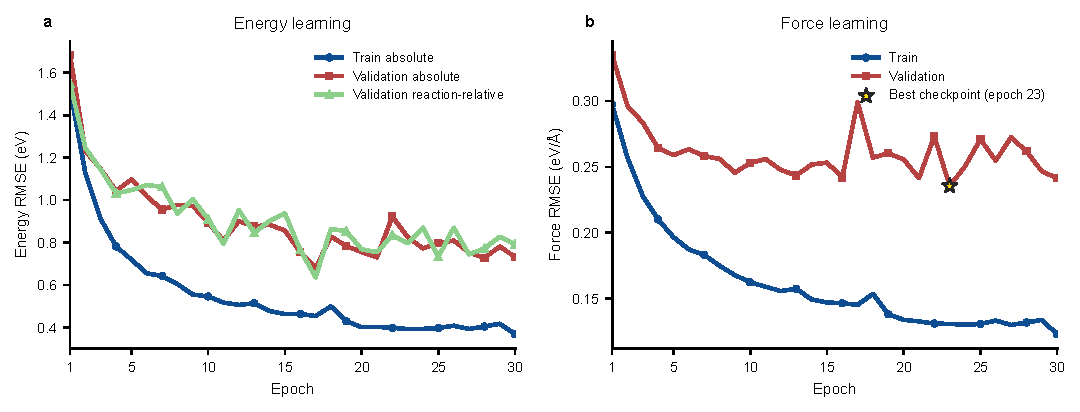
\includegraphics[width=\textwidth]{expanded_training_curves.pdf}
  \caption{Training and validation RMSE for the complete 30-epoch expanded-data run.
  The checkpoint with the lowest validation force RMSE occurs at epoch 23. Lines show
  one random seed and do not represent uncertainty across repeated runs.}
  \label{fig:training}
\end{figure}

At epoch 30, the training force RMSE is \SI{0.123}{eV\per\angstromunit}, while the
validation force RMSE is \SI{0.241}{eV\per\angstromunit}. The best validation force RMSE
is \SI{0.236}{eV\per\angstromunit} at epoch 23.

\begin{figure}[H]
  \centering
  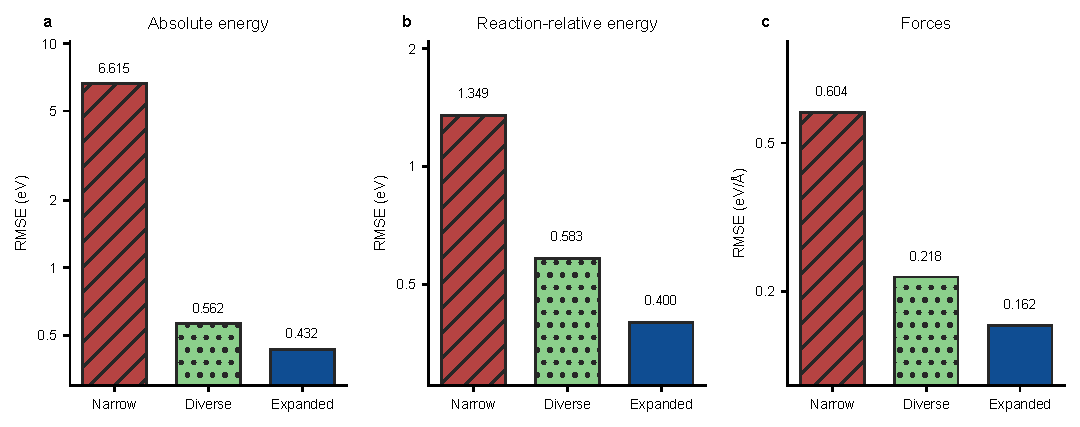
\includegraphics[width=\textwidth]{fixed_test_comparison.pdf}
  \caption{Fixed-test comparison of the three training strategies. All panels use a
  logarithmic vertical axis and the same held-out split. Lower values are better.}
  \label{fig:comparison}
\end{figure}

\begin{table}[H]
  \centering
  \caption{Metrics on the fixed test split. Force RMSE is calculated over Cartesian
  components.}
  \label{tab:results}
  \begin{tabular}{lccc}
    \toprule
    Training strategy & Absolute energy & Relative energy & Force \\
    & RMSE (eV) & RMSE (eV) & RMSE (eV/\AA) \\
    \midrule
    Narrow & 6.615 & 1.349 & 0.604 \\
    Diverse, equal size & 0.562 & 0.583 & 0.218 \\
    Expanded diverse & 0.432 & 0.400 & 0.162 \\
    \bottomrule
  \end{tabular}
\end{table}

At nearly equal configuration count, increasing coverage from 12 to 306 reactions
reduces absolute energy RMSE by approximately 91.5\%, reaction-relative energy RMSE
by 56.8\%, and force RMSE by 63.9\%. Expanding the diverse subset further reduces
these metrics by approximately 23\%, 31\%, and 26\%, respectively.


\section{Analysis and discussion}

\subsection{Energy and force optima do not coincide}

Epoch 17 gives the lowest validation absolute and relative energy errors in this run,
approximately \SI{0.680}{eV} and \SI{0.636}{eV}, but its validation force RMSE spikes
to \SI{0.299}{eV\per\angstromunit}. Epoch 23 instead minimizes validation force RMSE at
\SI{0.236}{eV\per\angstromunit}, while its validation energy errors are higher. Thus, a
small error in the value of an energy function does not guarantee a small error in
its derivative.

\subsection{Validation fluctuations and checkpoint selection}

Validation error is not optimized directly and need not decrease monotonically. The
late-stage fluctuations are consistent with a small validation split, stochastic
updates, a relatively large late-stage learning rate, and a growing generalization
gap. Recovery after individual spikes suggests optimization noise in addition to
overfitting. Because the intended downstream tasks include geometry and reaction-path
calculations, the current checkpoint is selected by validation force RMSE. A future
barrier-focused model should use a combined criterion that also protects relative
energy accuracy.

\subsection{Validation-test difficulty mismatch}

The best-checkpoint test force RMSE, \SI{0.162}{eV\per\angstromunit}, is substantially
lower than the best validation force RMSE. This does not by itself demonstrate
leakage. The two small subsets may differ in reaction difficulty, so per-reaction
error profiles are required before treating the aggregate test number as a robust
estimate of chemical generalization.


\bibliographystyle{unsrtnat}
\bibliography{references}
\end{document}
